% ==============================================================================
% reports/sections/results/06_05_port_ablation.tex
% ==============================================================================

\section{Kết quả thực nghiệm bóc tách cổng mạng}

Để kiểm chứng giả thuyết cho rằng mô hình gặp khó khăn trên tập Test theo thời gian chỉ đơn thuần là do dựa vào lối tắt cổng dịch vụ đích (\texttt{Destination Port}), nhóm tiến hành phân tích kịch bản bóc tách cổng (\texttt{without\_port}), trong đó đặc trưng này bị loại bỏ khỏi không gian huấn luyện.

Bảng \ref{tab:port_ablation} tổng hợp kết quả bóc tách cổng trên tập kiểm định $\Dval$.

% ==============================================================================
% reports/tables/generated/tab_port_ablation.tex
% ==============================================================================
\begin{table}[htbp]
\centering
\caption{Thực nghiệm Bóc tách Cổng mạng (Port Ablation) trên tập Validation phân tách theo thời gian.}
\label{tab:port_ablation}
\resizebox{\textwidth}{!}{%
\begin{tabular}{lrrrrr}
\toprule
\textbf{Mô hình} & \textbf{\FOne\ (Có Cổng)} & \textbf{\FOne\ (Không Cổng)} & \textbf{$\Delta$\FOne} & \textbf{SSH Recall (Có)} & \textbf{SSH Recall (Không)} \\
\midrule
Decision Tree & 0.7170 & 0.7169 & 0.0001 & 0.00\% & 0.00\% \\
Random Forest & 0.7181 & 0.7134 & 0.0047 & 0.00\% & 0.00\% \\
XGBoost & 0.7181 & 0.7136 & 0.0045 & 0.00\% & 0.00\% \\
\bottomrule
\end{tabular}%
}
\end{table}


Trên tập kiểm định $\Dval$, việc loại bỏ cổng làm giảm nhẹ điểm F1 của cả 3 mô hình (khoảng 0.0001 đến 0.0047), và tỷ lệ phát hiện tấn công SSH vẫn giữ ở mức 0.00\% (do mô hình tối ưu theo mẫu FTP chiếm đa số trong tập Val).

Khi quan sát kết quả trên tập kiểm thử $\Dtest$ theo thời gian (xem lại Phần A của Bảng \ref{tab:test_comparison}):
\begin{itemize}
    \item \textbf{Cây Quyết Định (Decision Tree)}: Điểm F1 tăng nhẹ từ 0.0000 lên \textbf{\DTTestWithoutPortFOne}, nhận diện được \DTTestWithoutPortSSHRecall\ tấn công SSH (7 mẫu).
    \item \textbf{Rừng Ngẫu Nhiên (Random Forest)}: Điểm F1 tăng từ \RFTestFOne\ lên \textbf{\RFTestWithoutPortFOne}, nhận diện được \RFTestWithoutPortSSHRecall\ tấn công SSH (14 trên tổng số 3,732 mẫu).
    \item \textbf{XGBoost}: Điểm F1 tăng từ 0.0000 lên \textbf{\XGBTestWithoutPortFOne}, nhận diện được \XGBTestWithoutPortSSHRecall\ tấn công SSH (13 trên tổng số 3,732 mẫu).
\end{itemize}

Sự thay đổi diện tích dưới đường cong ROC và đường cong Precision-Recall giữa hai kịch bản có và không có cổng được đối chiếu trực quan trên Hình \ref{fig:roc_pr_comparative}.

\begin{figure}[htbp]
\centering
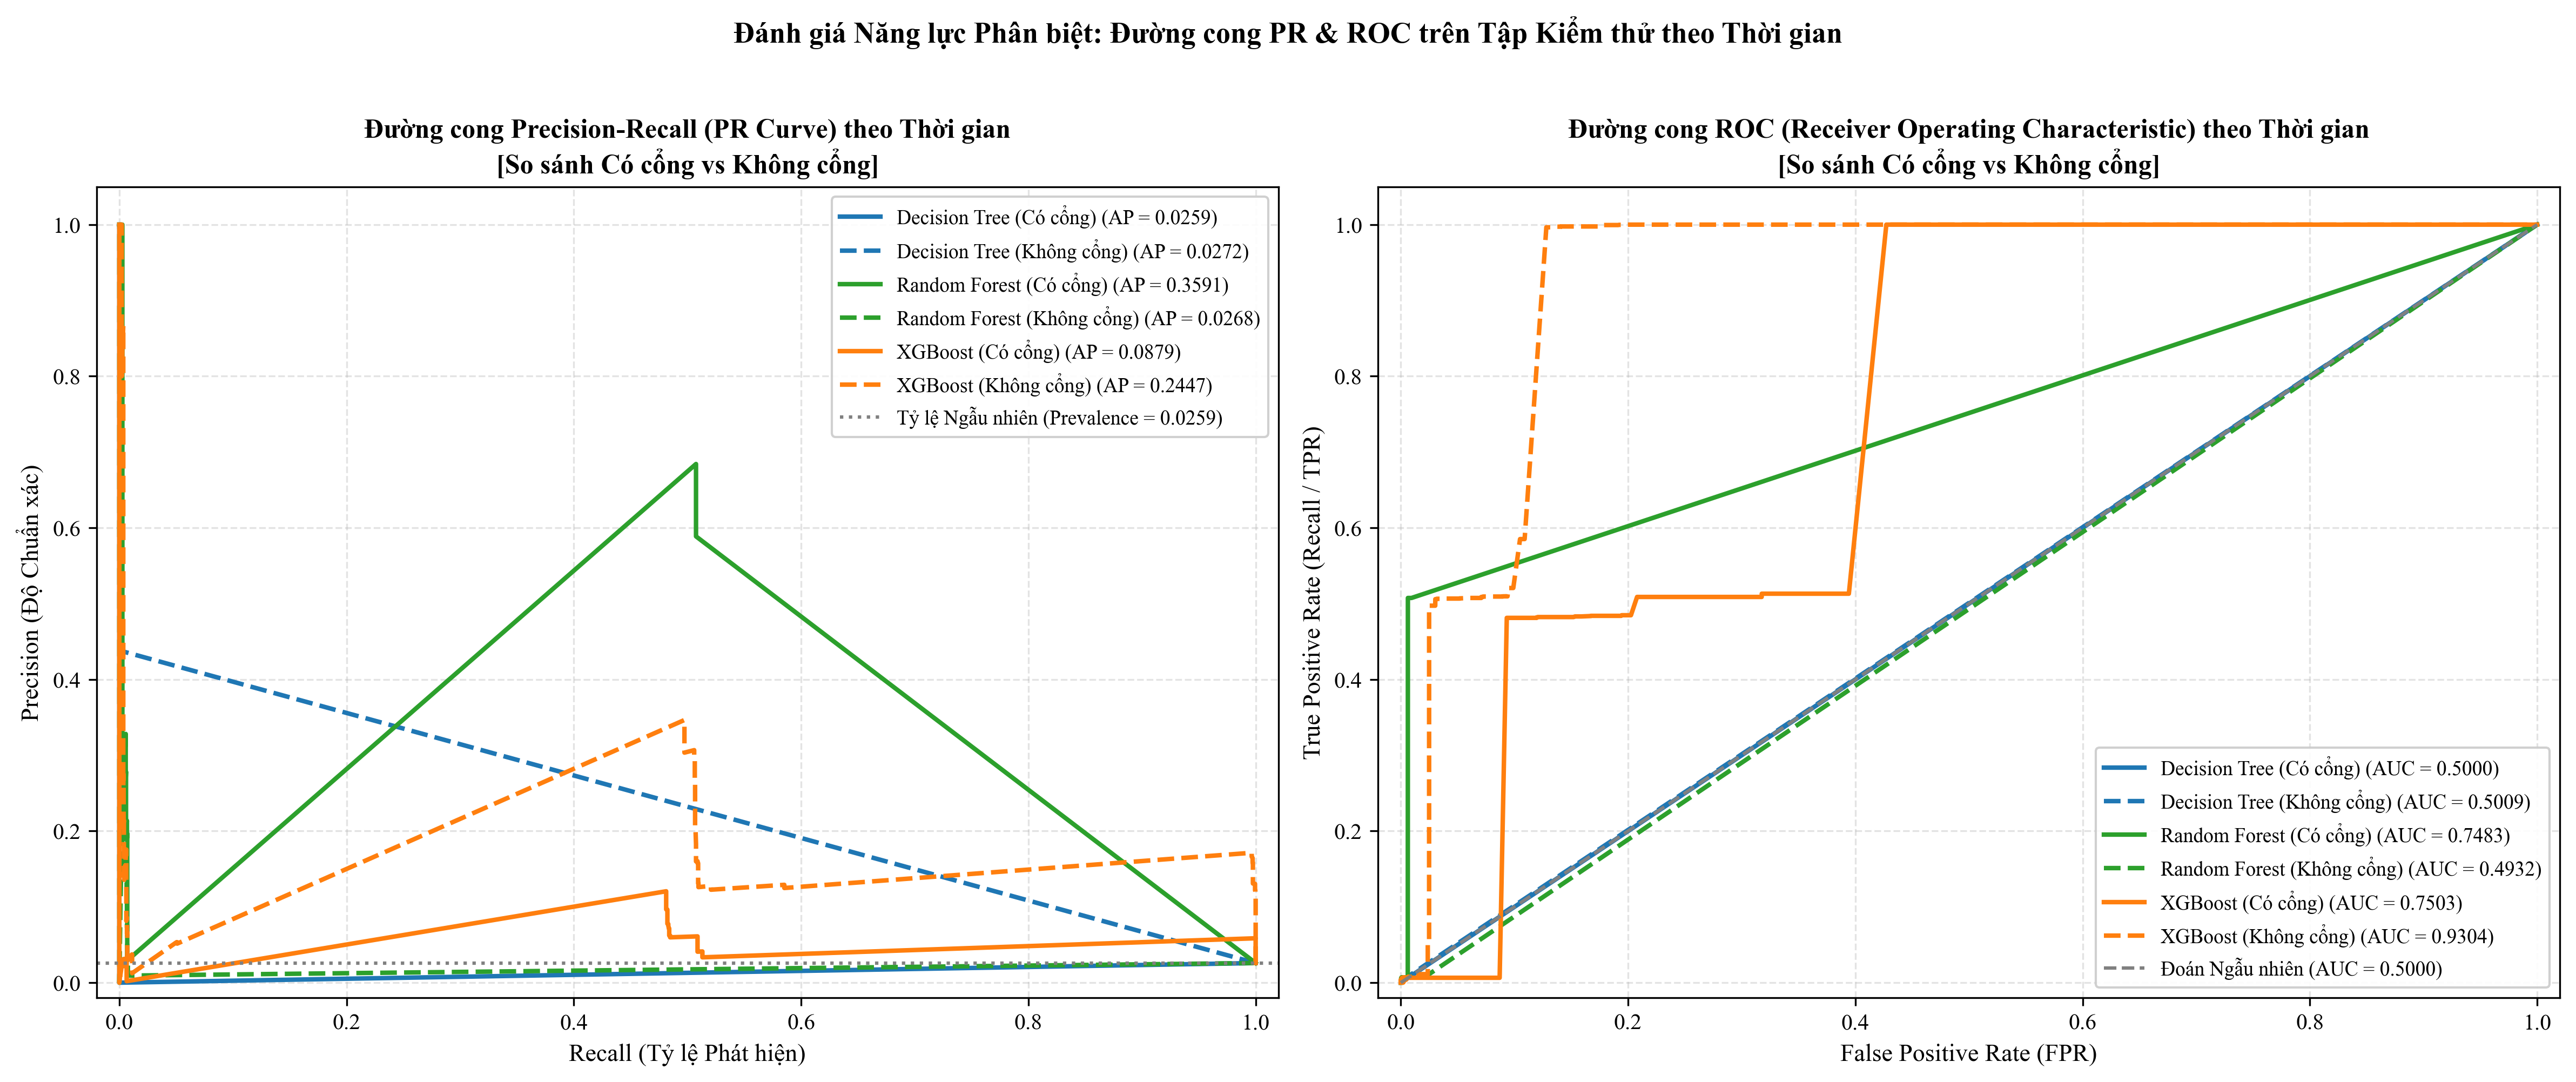
\includegraphics[width=0.92\textwidth]{experiments/figures/04_roc_and_pr_curves_comparative.png}
\caption{Đường cong ROC và Precision-Recall đối chiếu giữa các mô hình và kịch bản thực nghiệm, phản ánh sự biến thiên diện tích dưới đường cong khi có và không có đặc trưng cổng mạng.}
\label{fig:roc_pr_comparative}
\end{figure}

\noindent\textbf{Kết luận về vai trò của cổng dịch vụ:}
Việc loại bỏ cổng dịch vụ giúp các mô hình nhận diện được thêm một lượng nhỏ các flow SSH dựa trên đặc trưng hành vi (tỷ lệ SSH Recall tăng từ $0.00\% \text{ -- } 0.19\%$ lên $0.19\% \text{ -- } 0.38\%$).

Tuy nhiên, hiệu năng tổng thể của mô hình trong toàn bộ các tổ hợp theo thời gian vẫn ở mức rất thấp, với giá trị F1 cao nhất được ghi nhận là \textbf{\RFTestWithoutPortFOne} ở Random Forest (nhận diện được \RFTestWithoutPortSSHRecall\ tấn công SSH, tức 14/3,732 flow). Kết quả này cho thấy: mặc dù \texttt{Destination Port} là một lối tắt quan trọng của mô hình, việc loại bỏ cổng không đủ để giải quyết sự suy giảm hiệu năng tổng quát hóa. Nói cách khác, sự sụt giảm hiệu năng trong việc phát hiện SSH không thể được giải thích chỉ bằng riêng yếu tố cổng dịch vụ. Sự khác biệt về cơ chế hoạt động và phân phối đặc trưng thống kê gói tin giữa hai giao thức FTP và SSH (kết hợp với yếu tố thời gian và chiến dịch tấn công) là một cơ chế hợp lý góp phần tạo nên sự dịch chuyển phân phối này.
